\subsubsection*{Análise e Interpretação dos Resultados - Merge Sort}

\qquad A análise do \textit{Merge Sort} é mais direta que a dos algoritmos anteriores, pois seu comportamento não depende da ordem inicial dos dados. Em qualquer vetor, o algoritmo divide o trecho ao meio até chegar a elementos individuais e depois intercala as partes. Como o número de divisões e o custo das intercalações são sempre os mesmos, o desempenho é o mesmo nos três casos \cite{sedgewick}.

\qquad Para ilustrar o funcionamento do algoritmo, a Figura \ref{fig:merge_teste_mesa} apresenta um teste de mesa com um vetor de sete elementos. Como o vetor tem tamanho ímpar, a metade esquerda recebe um elemento a mais, o que reflete o cálculo do ponto médio feito no código. A parte superior da figura mostra a divisão e a parte inferior mostra as intercalações.

\begin{figure}[htbp]
    \centering
    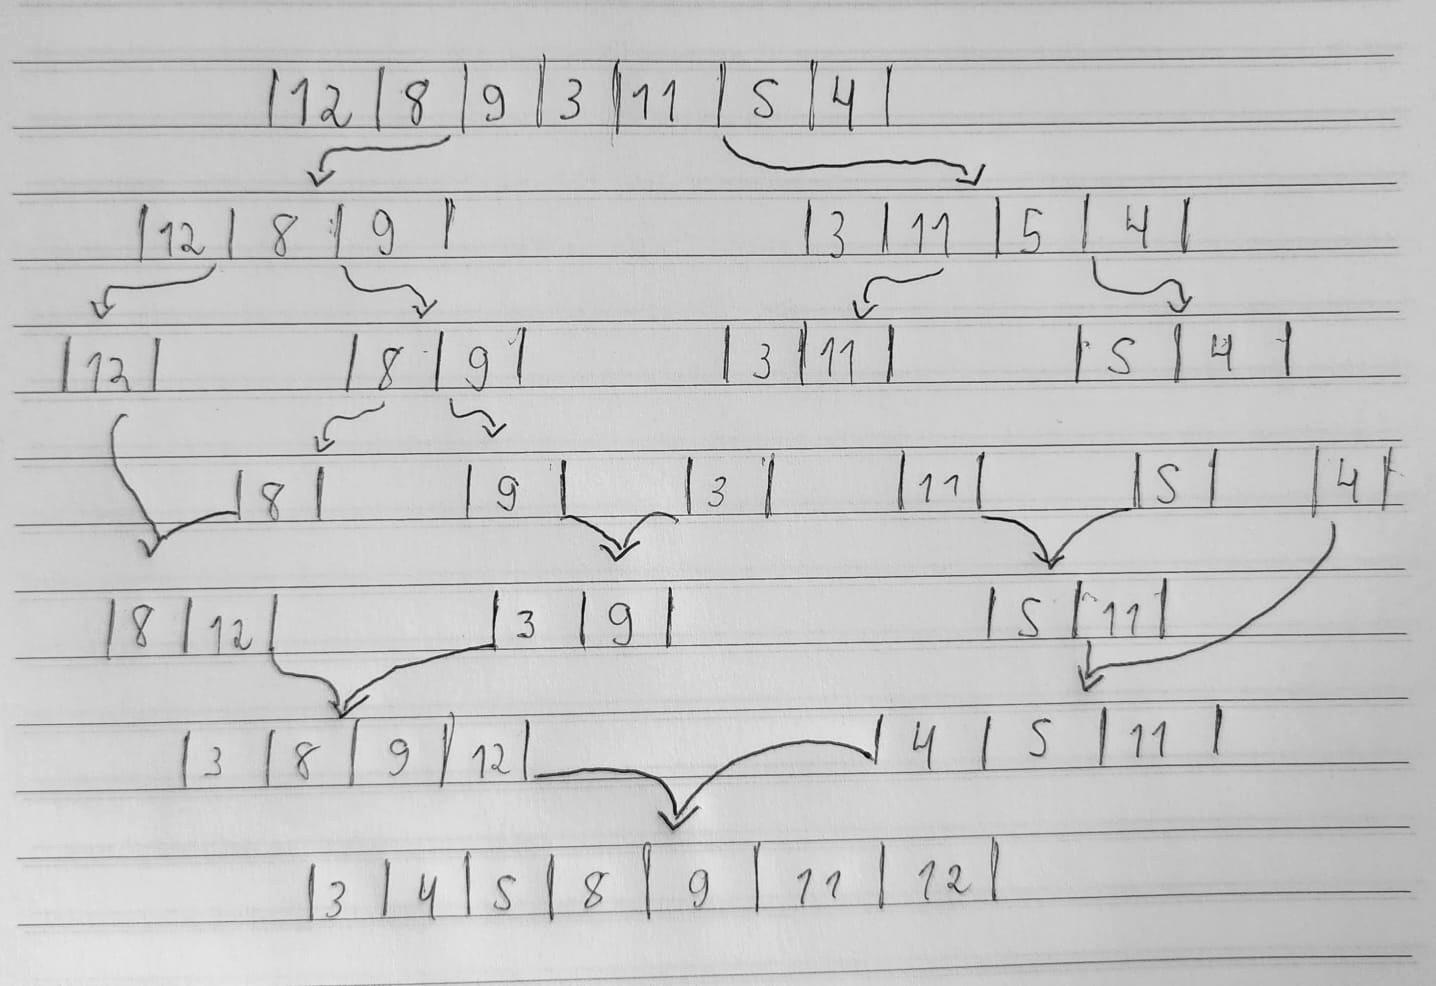
\includegraphics[width=0.9\textwidth]{Imagens/Merge Sort/mergeteste.jpeg}
    \caption{Teste de mesa do \textit{Merge Sort} para um vetor de sete elementos (elaborado pelo autor).}
    \label{fig:merge_teste_mesa}
\end{figure}

\FloatBarrier

\qquad Para obter a complexidade, usa-se a recorrência do algoritmo. O tempo $T(n)$ para ordenar $n$ elementos é a soma do custo constante de calcular o ponto médio, do tempo das duas chamadas recursivas sobre metades do vetor e do custo da intercalação, que é $\Theta(n)$, como visto na análise do código. Isso resulta em $T(n) = 2T(n/2) + n$. A Figura \ref{fig:merge_recorrencia} mostra o desenvolvimento dessa recorrência por expansão, considerando $n = 2^k$.

\begin{figure}[htbp]
    \centering
    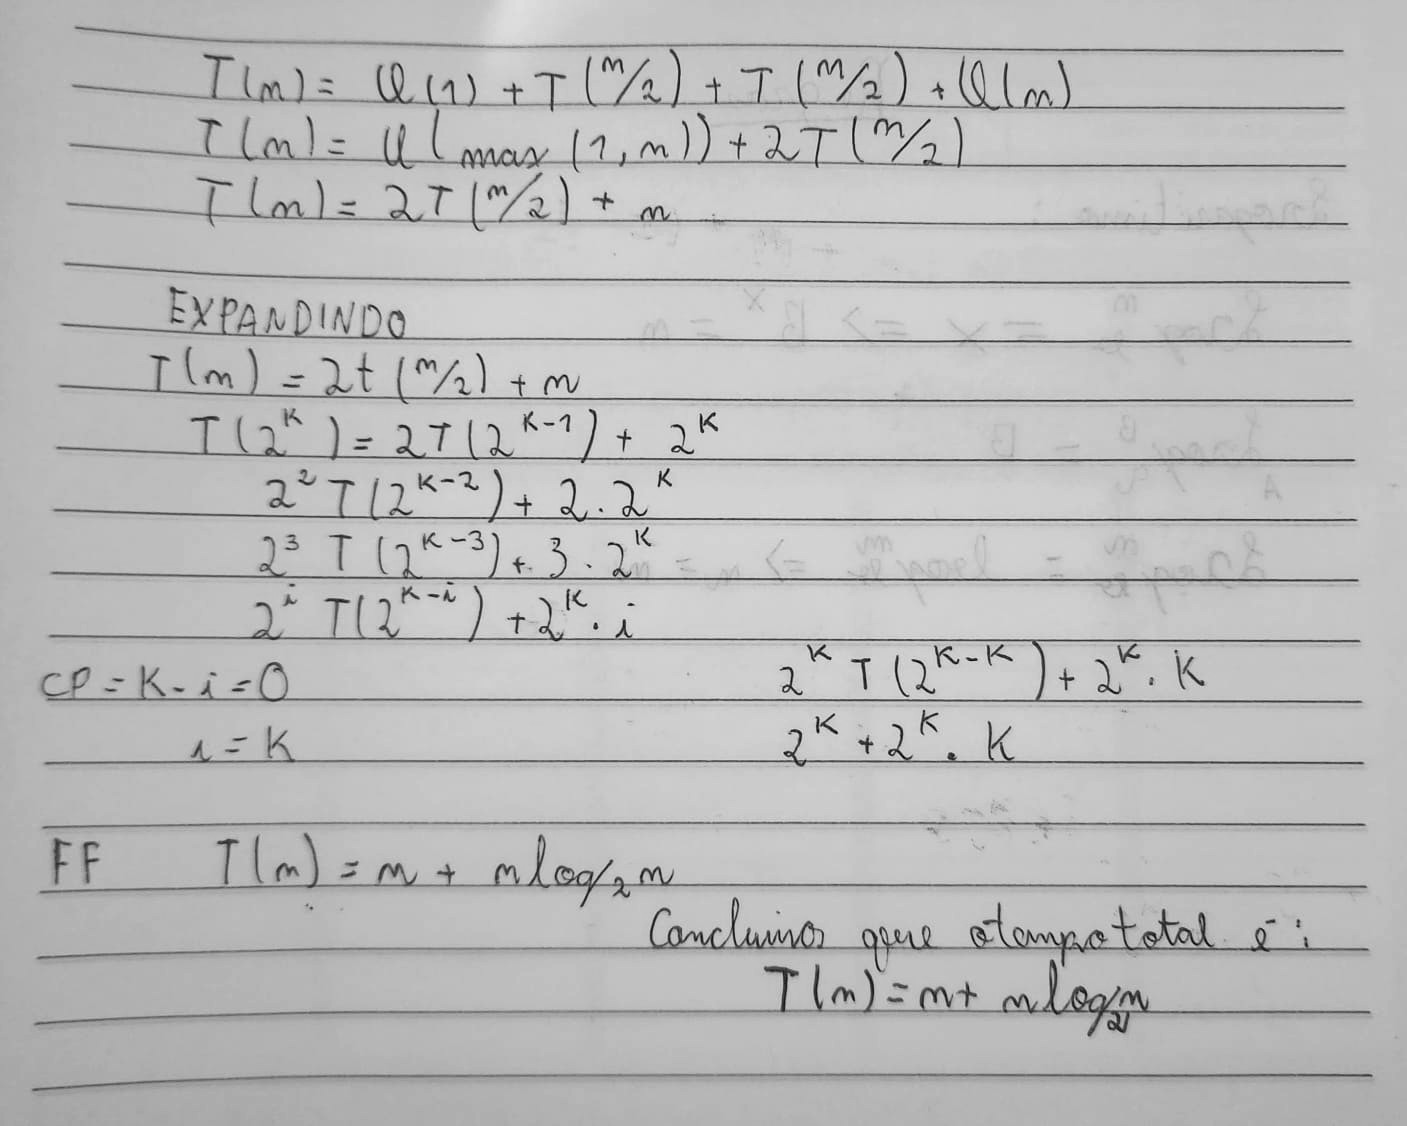
\includegraphics[width=0.8\textwidth]{Imagens/Merge Sort/mergecalculo.jpg}
    \caption{Resolução da recorrência do \textit{Merge Sort} por expansão (elaborado pelo autor).}
    \label{fig:merge_recorrencia}
\end{figure}


\qquad Ao expandir a recorrência, cada nível acrescenta o termo $2^k$ ao custo. Isso acontece porque, a cada nível, o número de subproblemas dobra e o tamanho de cada um cai pela metade, de modo que o total de elementos intercalados por nível continua sendo $n$. A expansão termina quando $k - i = 0$, ou seja, $i = k$, e o resultado é $T(n) = 2^k + 2^k \cdot k$. Como $n = 2^k$, tem-se $k = \log_2 n$, e portanto
\[
T(n) = n + n \log_2 n .
\]
Esse resultado mostra que o tempo total é $O(n \log n)$. Os principais casos de desempenho são:
\begin{itemize}
    \item \textbf{Melhor caso:} $O(n \log n)$. Mesmo com o vetor já ordenado, o algoritmo faz todas as divisões e todas as intercalações, pois não existe verificação que permita interromper o processo mais cedo.

    \item \textbf{Pior caso:} $O(n \log n)$. A altura da árvore de chamadas é sempre $\log_2 n$, e cada nível custa $n$ em qualquer ordem dos dados. Diferente do \textit{Bubble Sort} e do \textit{Selection Sort}, o pior caso não chega a $O(n^2)$.

    \item \textbf{Caso médio:} $O(n \log n)$, pelo mesmo motivo dos casos anteriores.
\end{itemize}

\qquad Os tempos medidos nos testes são compatíveis com essa análise. Ao aumentar a entrada de 100.000 para 1.000.000 de elementos (10 vezes maior), o tempo do caso aleatório passou de 0,023 para 0,292, um crescimento de cerca de 12,7 vezes. Para $n \log n$, o crescimento esperado nessa mudança é de aproximadamente 12 vezes, enquanto em um algoritmo quadrático seria de 100 vezes. Nos vetores crescentes e decrescentes o crescimento foi de cerca de 11 e 9 vezes, respectivamente. Os tempos dos três tipos de entrada ficaram próximos entre si, o que confirma que o \textit{Merge Sort} não depende da ordem inicial dos dados. A diferença entre eles vem de detalhes de execução, como o número de comparações feitas em cada intercalação e o uso do \textit{cache} do processador.

\qquad Quanto à \textbf{complexidade de espaço}, o \textit{Merge Sort} utiliza $O(n)$, devido ao vetor auxiliar de $n$ posições usado nas intercalações, além de $O(\log n)$ para a pilha de chamadas recursivas. Por isso, diferente dos demais algoritmos deste trabalho, ele não é \textit{in-place}. Em troca desse espaço extra, ele garante o desempenho $O(n \log n)$ em todos os casos e é estável.